\documentclass[aspectratio=169]{beamer}
\usetheme{metropolis}

\usepackage{algorithm,algpseudocode}
\usepackage{listings}
\usepackage{graphicx}

\title{Présentation - Implémentation d’un langage de programmation logique d’ordre supérieur avec MALI}
\subtitle{Pascal Brisset, Novembre 1989}
\date{\today}
\author{David Sreng, Basile Pesin}
\institute{Faculté des Sciences de Sorbonne Université}

\begin{document}

\lstdefinelanguage{lprolog}{%
   columns=fullflexible,%
   % keywordstyle=\bfseries,
   commentstyle=\slshape,%
   keywords={%
    type
   },%
   keywordstyle={\color{blue}\sffamily},%
   morekeywords=[2]{%
     list
   },%
   keywordstyle=[2]{\color{black}\sffamily},%
   classoffset=2,%
   sensitive,%
   comment=[l]\#,%
   morestring=[d]",%"
   escapechar=\$,
   literate=*{->}{{$\rightarrow$}}1
   {\\}{{\color{blue}\sffamily$\lambda$}}1
   {=>}{{$\Rightarrow$}}1,%
   showlines=true,
   frame=single,
}[keywords,comments,strings]%

\lstset{basicstyle=\tt\footnotesize, frame=single}

\maketitle

\begin{frame}{Motivations}
  En 1989, l'interpréteur de $\lambda$-Prolog existant est écrit en Prolog, pas efficace pour des programmes réels

  Développement d'un compilateur pour le langage Z, restriction de $\lambda$-Prolog:
  \begin{itemize}
    \item utilise des $\lambda$-termes typés
    \item unification d'ordre supérieure
    \item quantification universelle
  \end{itemize}
\end{frame}

\section{L'algorithme d'Huet}

\begin{frame}{Données en entrée}
  Travaille sur des $\lambda$-termes bien typés
  \begin{itemize}
    \item $\eta$-expansés: $e \equiv \lambda x.(e x)$ (tous les corps d'abstractions de type atomiques)
    \item $\beta$-réduits: $(\lambda x . e_1) e_2 \equiv e_1[e_2/x]$
  \end{itemize}
  Donc sous forme normale de tête : $\lambda x_1 \ldots x_n . (@ e_1 \ldots e_p)$

  Une expression est flexible si la tête $@$ est une inconnue, rigide sinon
\end{frame}

\begin{frame}{SIMPL}
  Avec un ensemble de paires à unifier $<e_1, e_2>$:
  \begin{algorithmic}
    \Procedure{SIMPL}{}
    \If{$n = \emptyset$} (succès, $\emptyset$)
    \EndIf
    \State{TRIVIAL : unifier une paire $<var, expr>$ si trouvée, et reprendre}
    \If{il n'y a pas de paire rigide-rigide} (succès, n)
    \EndIf
    \If{il y en a une $<\lambda x_1 \ldots x_n . (@_1 e_1^1 \ldots e_{p_1}^1), \lambda x_1 \ldots x_n . (@_2 e_1^2 \ldots e_{p_2}^2)>$}
    \If{$@_1 \neq @_2$} (échec, $\emptyset$)
    \Else
    \State{Ajouter les $<\lambda x_1 \ldots x_n . e_i^1, \lambda x_1 \ldots x_n . e_i^2>$ à $n'$}
    \EndIf
    \EndIf
    \EndProcedure
  \end{algorithmic}
\end{frame}

\begin{frame}{MATCH}
  Avec une paire flexible-rigide $<\lambda x_1 \ldots x_n . (v e_1^1 \ldots e_{p_1}^1), \lambda x_1 \ldots x_n . (@ e_1^2 \ldots e_{p_2}^2)>$\\
 et avec $E_i$ = $(h_i w_1 \ldots w_{p_1})$, $h_i$ sont des nouvelles inconnues
  \begin{algorithmic}
    \Procedure{MATCH}{}
    \If{$@$ est une constante}
    \State{imitation : $<v, \lambda w_1 \ldots w_{p_1} . (@ E_1 \ldots E_{p_2})>$}
    \EndIf
    \For{$i$, si $e_i^1$ : $\gamma_1 \rightarrow \ldots \rightarrow \gamma_r \rightarrow \beta$ ($\beta$ type de retour de $v$)}
    \State{projection : $<v, \lambda w_1 \ldots w_{p_1} . (w_i E_1 \ldots E_r)>$}
    \EndFor
    \EndProcedure
  \end{algorithmic}

  Phase non déterministe ! On génére plusieurs possibilités de substitutions à explorer
\end{frame}

\begin{frame}{Déroulement de l'algorithme}
  Construction d'un arbre pour les termes $<e_1, e_2>$
  \begin{algorithmic}
    \Procedure{Unification}{}
    \State{$root = SIMPL(<e_1, e_2>)$}
    \While{il reste un noeud $p$ flexibles-rigide}
    \State{$\Sigma = MATCH(p)$}
    \State{On choisit $\sigma \in \Sigma$, et on fait $SIMPL(\sigma(p))$ pour obtenir un nouveau fils}
    \EndWhile
    \EndProcedure
  \end{algorithmic}
\end{frame}

\section{Implémentation dans MALI}

\begin{frame}{MALI}
  \textbf{Machine Adaptée aux Langages Indéterministes}
  \begin{itemize}
    \item Implémentée en C
    \item Avec GC
    \item Abstrait la pile de recherche (en profondeur)
    \item Représentation et parcours de termes
  \end{itemize}
\end{frame}

\begin{frame}{Chaîne de compilation}
  \begin{center}
    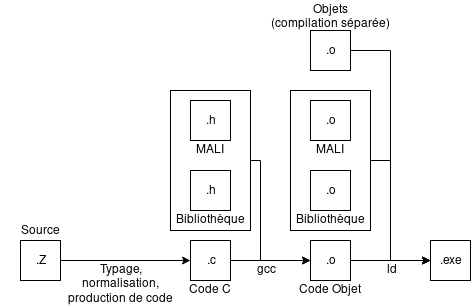
\includegraphics[width=.5\paperwidth]{assets/mali-chain.png}
  \end{center}
\end{frame}

\begin{frame}{Compilation}
  Etapes de compilation:
  \begin{enumerate}
  \item Typage (et annotation) des termes
  \item $\eta$-expansion statique
  \item $\beta$-réduction statique
  \item Production du code C (exemple plus loin)
  \end{enumerate}
  Compilateur écrit en Prolog, plus tard bootstrappé en Z.

  ! Des phases d'expansions et de réduction dynamiques sont aussi nécessaires !
\end{frame}

\begin{frame}{Représentation des données}
  La machine utilise une désignation (tas) : $Nom \rightarrow Terme$
  avec le $Nom$ contenant la $Nature$ et la $Sorte$ (type)
  \begin{table}
  \begin{tabular}{l|l|l}
    Structure & Usage & Opérations\\
    \hline
    Atome & constantes, types atomiques & $Atom$ (construction) \\
    Construit & types construits & $Cons$, $Car$, $Cdr$\\
    N-uplet & abstractions, applications & $Nth$\\
    Variable & variables, inconnue de type & $Substituer$\\
    Variable à Attribut & abstractions, applications, inconnues & $SubstituerA$\\
    \hline
  \end{tabular}
  \end{table}
\end{frame}

\begin{frame}{Pourquoi la variable à attribut ?}
  On fait des $\beta$-réduction et $\eta$-expansion dynamique $\rightarrow$ réécritures (qui doivent pouvoir être renversées lors d'un retour arrière)

  \begin{itemize}
    \item stocker un terme $t$ à réécrire dans une v.a. $x_t$ (au parcours on lira $t$)
    \item si on doit réécrire $t \rightarrow t'$ on fait $substituer(x_t, t')$
    \item alors au parcours de terme on lira $t'$
    \item en cas de retour arrière, la substitution est automatiquement défaite
  \end{itemize}

  + v.a. utilisée pour stocker des informations (type des variables)
\end{frame}

\begin{frame}[fragile]{Exemple de code C produit}
  \begin{lstlisting}[language=lprolog]
    type concat list A -> list A -> list A -> o.
    concat [] X X.
    concat [X|XS] Y [X|Z] :- concat XS Y Z.
  \end{lstlisting}

  \begin{lstlisting}[language=C,keywordstyle=\color{blue}\ttfamily]
    typedef struct { Nom x; Nom y; Nom z; } concat_st;

    void concat_proc1(concat_st *c) {
      Unifier(c->x, Nil); Unifier(c->y, c->z);
    }

    void concat_proc2(concat_st *c) {
      Nom x = Variable(); Nom xs = Variable(); Nom z = Variable();
      Unifier(c->x, Cons(x, xs)); Unifier(c->z, Cons(x, z));
      concat_st *c1 = malloc(); c1->x = xs; c1->y = c->y; c1->z = z;
      Resoudre(c1);
    }
  \end{lstlisting}
\end{frame}

\begin{frame}{Exécution}
  Depth-first search (appel à $Resoudre$ indeterministe, comme pour Prolog).

  Pile de recherche (contient l'état et les choix faits dans les cas indeterministes) avec opérations
  \begin{itemize}
    \item $Sauvegarder$ : Avant chaque instantiation d'une variable
    \item $Reprendre$ : Au retour arrière, dépile un niveau de la pile
  \end{itemize}
\end{frame}

\begin{frame}{Spécificités de $\lambda$-Prolog}
  SIMPL (déterministe) est écrite en C

  MATCH (indéterministe) est implémenté dans le langage source ($\lambda$-Prolog / Z) avec Imitation et Projection des prédicats déterministes donnés.

  \textbf{MATCH est bootstrap comme un ensemble de clauses du langage source}
\end{frame}

\begin{frame}{Gestion de la mémoire}
  Les substitutions sont coûteuses en espace (+ réécritures)

  Opération $Reduire : Nom \rightarrow Nom$ : le paramètre est le $Nom$ du terme principal à garder (les autres termes utiles sont trouvés par parcours). Après la procédure, la désignation ne contient que le nom résultat.

  On peut libérer:
  \begin{itemize}
    \item Les termes non protégés par $Reduire$, et non sauvegardés
    \item Les termes sauvegardés dans sous-piles de recherches détruites (par retour-arrière ou cut)
  \end{itemize}
\end{frame}

\section{Conclusion}

\begin{frame}{Extensions de l'article}
  L'article décrit une implémentation efficace d'un langage dérivé de $\lambda$-Prolog.

  Manquent pour une implémentation complète de $\lambda$-Prolog:
  \begin{itemize}
    \item Implication (ajout dynamique de clauses)
    \item Polymorphisme
    \item Plus d'optimisations
  \end{itemize}
\end{frame}

\begin{frame}{A retenir pour le projet}
  \begin{itemize}
    \item Unification (Algorithme de Huet)
    \item Structures de données (pile de recherche)
    \item $\eta$-expansion dynamique nécessaire
    \item Garbage collector ? (en fonction du langage utilisé)
  \end{itemize}
\end{frame}

\end{document}
